\chapter{Reactivity Feedback Mechanisms}
\label{ch:feedback}

Feedback is where thermal physics re-enters the neutron economy. This chapter
defines the feedback coefficients, derives the dominant mechanisms---Doppler,
moderator/coolant temperature, and void---and establishes the signs that decide
stability. The void coefficient receives special attention because its sign is
the crux of the Chernobyl story.

\section{Temperature coefficients of reactivity}

A \textbf{temperature coefficient of reactivity} is the change in reactivity per
unit change in some temperature,
\begin{equation}
\alpha_T = \frac{\partial \rho}{\partial T}.
\end{equation}
There is one for each material whose temperature affects the neutron economy:
$\alpha_D=\partial\rho/\partial \Tf$ (the fuel or Doppler coefficient),
$\alpha_M=\partial\rho/\partial T_M$ (the moderator coefficient), and analogously
for coolant and structure. For stability, the sign is paramount: a
\emph{negative} coefficient means that heating removes reactivity, which opposes a
power rise---stabilising. A \emph{positive} coefficient means heating adds
reactivity, reinforcing a power rise---destabilising.

\begin{definition}[Power coefficient]
The \textbf{power coefficient} $\alpha_P=\partial\rho/\partial P$ aggregates all
temperature feedbacks weighted by how strongly each temperature responds to
power:
\begin{equation}
\alpha_P = \alpha_D\frac{\partial \Tf}{\partial P}
         + \alpha_M\frac{\partial T_M}{\partial P}
         + \alpha_v\frac{\partial \bar v}{\partial P} + \cdots
\end{equation}
A negative power coefficient is the single most important guarantee of inherent
stability: it means that any increase in power is self-limiting. Western power
reactors are designed and licensed to have a negative power coefficient across
the operating range.
\end{definition}

\section{The Doppler effect: prompt and reliably negative}

The Doppler coefficient is the reactor's fastest and most dependable feedback. It
arises from the broadening of the neutron-capture resonances of $^{238}$U (and
$^{240}$Pu) as the fuel heats.

At a resonance, the absorption cross-section is sharply peaked at a resonance
energy $E_0$. The thermal motion of the absorbing nuclei---greater at higher
temperature---Doppler-shifts the relative neutron energy, smearing the resonance
into a broader, lower peak while approximately conserving its area
(Figure~\ref{fig:doppler}). The key consequence is that broadening \emph{reduces
self-shielding}: when the resonance is narrow and tall, neutrons at the resonance
energy are absorbed in the thin outer layer of the fuel and the interior is
``shielded''; when the resonance is broadened, more of the fuel volume
participates in absorption. Net resonance absorption therefore \emph{increases}
with temperature, the resonance escape probability $p$ \emph{falls}, and
reactivity \emph{decreases}.

\begin{figure}[H]
\centering
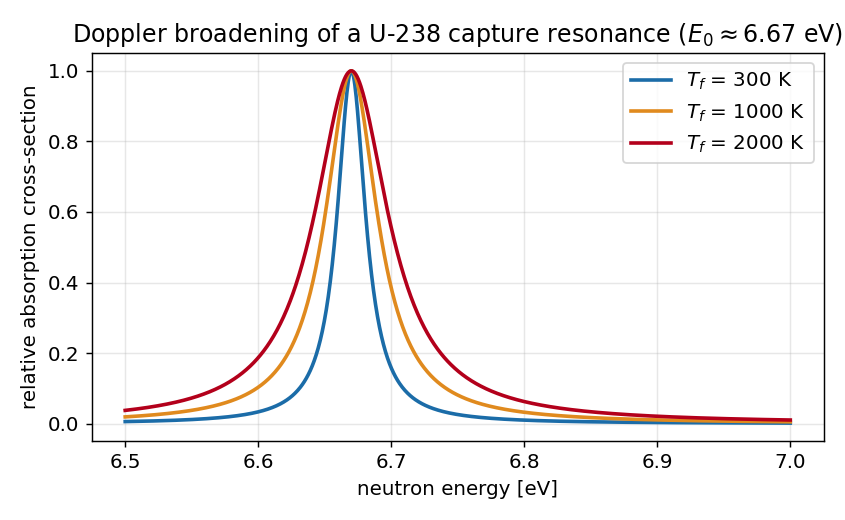
\includegraphics[width=0.74\linewidth]{figures/doppler.png}
\caption{Doppler broadening of a $^{238}$U capture resonance with increasing fuel
temperature. The peak lowers and widens at roughly constant area; reduced
self-shielding increases net resonance absorption, lowering reactivity. This is
the prompt, negative Doppler feedback.}
\label{fig:doppler}
\end{figure}

Two features make Doppler feedback uniquely valuable. First, it is \emph{prompt}:
it depends on the fuel temperature, which rises essentially instantly with power,
so it acts even on a prompt-critical excursion. Second, it is \emph{reliably
negative} in any fuel containing a fertile resonance absorber such as $^{238}$U,
which is to say in essentially all power-reactor fuel. A useful approximate form
is
\begin{equation}
\alpha_D \approx \frac{A}{\sqrt{\Tf}},\qquad
\Delta\rho_D = \int \alpha_D\,\dd \Tf \propto \sqrt{\Tf},
\end{equation}
with $A<0$; the $1/\sqrt{\Tf}$ dependence means the coefficient weakens at high
temperature but never changes sign. It was the absence of a sufficiently strong
\emph{net} prompt negative feedback, not the absence of Doppler per se, that
doomed the RBMK: the RBMK had Doppler feedback, but at low power its huge positive
void coefficient overwhelmed it.

\keypoint{Doppler feedback is prompt and negative. It is the only feedback fast
enough to limit a prompt-critical excursion, and it is the physical reason a
well-designed reactor ``rides out'' a reactivity insertion. The decisive question
for any reactor is whether the prompt feedback is \emph{net} negative once the
void coefficient is included.}

\section{Moderator and coolant temperature feedback}

In a thermal reactor the moderator slows neutrons to thermal energies. Its
temperature affects reactivity through two competing routes: changes in moderator
\emph{density} (a hotter, less dense moderator slows neutrons less effectively),
and changes in the thermal neutron \emph{spectrum} (a hotter moderator hardens
the spectrum, shifting absorption rates). In a light-water reactor the density
effect dominates, and because water is both moderator and coolant, heating it
reduces moderation. Whether this raises or lowers reactivity depends on whether
the lattice is under- or over-moderated:

\begin{itemize}[nosep]
\item In an \textbf{under-moderated} lattice (PWR design intent), there is ``too
little'' moderation at the optimum; reducing it further (by heating/expanding the
water) lowers reactivity. The moderator temperature coefficient (MTC) is
\emph{negative}---stabilising.
\item In an \textbf{over-moderated} lattice, reducing moderation moves toward the
optimum and \emph{raises} reactivity. The MTC is positive---destabilising.
\end{itemize}

Light-water reactors are deliberately designed under-moderated to guarantee a
negative MTC. The moderator coefficient acts with the coolant transport delay
and so governs the slower stability of the operating point rather than the prompt
excursion.

\section{The void coefficient}

When coolant boils (in a BWR, or in any reactor during a transient) or flashes to
steam, it forms \emph{voids}---regions of vapour with much lower density than
liquid. The \textbf{void coefficient} $\alpha_v=\partial\rho/\partial \bar v$,
where $\bar v$ is the void fraction, captures the reactivity effect. Voiding has
several effects at once: it removes moderator (in a water-moderated reactor), it
removes a neutron absorber (water absorbs neutrons), and it changes leakage. The
net sign depends, once again, on whether the lattice is under- or
over-moderated.

\begin{itemize}[nosep]
\item In an \textbf{under-moderated} water reactor (PWR, BWR), the loss of
moderation dominates: voiding lowers reactivity, $\alpha_v<0$---stabilising. A
BWR runs with boiling by design, and its negative void coefficient is the basis
of its self-regulation (and, in fast transients, of a mild instability tendency
discussed in Chapter~\ref{ch:linear}).
\item In the \textbf{RBMK}, moderation was provided primarily by \emph{graphite},
which is unaffected by boiling the water. The water acted mainly as coolant and
as a parasitic \emph{absorber}. Voiding the water therefore removed an absorber
without removing much moderation, so reactivity \emph{rose}: $\alpha_v>0$,
strongly so, and most strongly at low power where the steam fraction was small and
sensitive. This is the single most important design fact behind Chernobyl.
\end{itemize}

\begin{figure}[H]
\centering
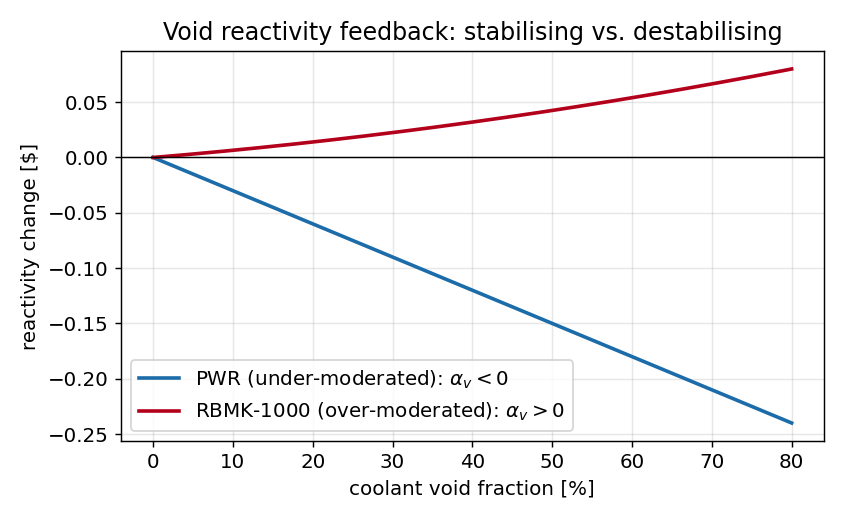
\includegraphics[width=0.74\linewidth]{figures/void.png}
\caption{Void reactivity feedback for an under-moderated lattice (PWR, negative
slope) and an over-moderated lattice (RBMK-1000, positive slope). The void
coefficient is the slope at the operating point; its sign decides whether boiling
is self-limiting or self-amplifying.}
\label{fig:void2}
\end{figure}

\begin{remark}[The vicious circle of a positive void coefficient]
A positive void coefficient creates a runaway loop: power up $\to$ more boiling
$\to$ more voids $\to$ \emph{more} reactivity $\to$ more power. If the prompt
Doppler feedback is not strong enough to overcome it, the loop is unstable. At
the RBMK's low-power, low-flow state on the night of the accident, the loop gain
exceeded unity and the prompt feedback was net positive---a condition the machine
should never have been allowed to enter.
\end{remark}

\section{Other feedbacks: expansion, bowing, and burnup}

Several smaller effects round out the picture. \emph{Thermal expansion} of fuel,
cladding, and structure changes geometry and hence leakage and lattice spacing;
in fast reactors, fuel and structural expansion provide important negative
feedback. \emph{Fuel bowing} and \emph{control-rod-bank expansion} can contribute
small coefficients. Over the long term, \emph{burnup} changes the isotopic
composition and hence all coefficients---a reactor's MTC, for example, becomes
more negative as soluble boron is reduced over a cycle. For the fast dynamics of
stability, however, the trio of Doppler, moderator, and void dominate, and the
contest between prompt-negative Doppler and a possibly-positive void coefficient
is the essential drama.

\section{Assembling the feedback reactivity}

For the coupled model we write the total reactivity as the externally imposed part
plus the feedback,
\begin{equation}
\rho(t) = \rho_{ext}(t)
        + \alpha_D\,[\Tf(t)-\Tf^0]
        + \alpha_M\,[\Tc(t)-\Tc^0]
        + \alpha_v\,[\bar v(t)-\bar v^0] + \cdots
\label{eq:rho-feedback}
\end{equation}
Substituting \eqref{eq:rho-feedback} into the point kinetics
\eqref{eq:prk} and coupling to the thermal equations of
Chapter~\ref{ch:thermal} closes the loop. The resulting nonlinear system is the
subject of Chapter~\ref{ch:coupled} and of the stability analysis of Part~III. Its
behaviour hinges entirely on the signs and magnitudes of the coefficients in
\eqref{eq:rho-feedback}: a system with net-negative, suitably prompt feedback is
stable and self-regulating; a system with net-positive feedback, especially a
prompt one, is an accident waiting for a trigger.



\section{Rigorous theory of the Doppler coefficient}
\label{sec:doppler-rigorous}

We derive the temperature dependence of the Doppler coefficient from
resonance-absorption theory. Near an isolated resonance at $E_0$ the capture
cross-section of a \emph{stationary} target is the Breit--Wigner form
\begin{equation}
\sigma_\gamma^0(E)=\sigma_0\,\frac{\Gamma_\gamma}{\Gamma}\sqrt{\frac{E_0}{E}}\,
\frac{1}{1+x^2},\qquad x=\frac{2(E-E_0)}{\Gamma},
\end{equation}
with total width $\Gamma$, radiative width $\Gamma_\gamma$, and peak $\sigma_0$.
Thermal motion of the target nuclei convolves this with a Maxwellian of relative
velocities, giving the Doppler-broadened shape
\begin{equation}
\sigma_\gamma(E,T)=\sigma_0\,\frac{\Gamma_\gamma}{\Gamma}\sqrt{\frac{E_0}{E}}\,
\psi(\xi,x),\qquad
\psi(\xi,x)=\frac{\xi}{2\sqrt{\pi}}\!\int_{-\infty}^{\infty}\!
\frac{e^{-\frac14\xi^2(x-y)^2}}{1+y^2}\,\dd y,
\label{eq:psi}
\end{equation}
with broadening parameter $\xi=\Gamma/\Delta_D$ and \emph{Doppler width}
\begin{equation}
\Delta_D=\sqrt{\frac{4E_0 k_B T}{A}}\ \propto\ \sqrt{T},
\label{eq:dopplerwidth}
\end{equation}
$A$ the target mass number. The convolution \eqref{eq:psi} conserves area,
$\int_{-\infty}^{\infty}\psi\,\dd x=\pi$, so broadening lowers and widens the line
without changing its integral.

The reactivity effect operates through the \emph{effective resonance integral}
under self-shielding. In the narrow-resonance approximation with background
cross-section $\sigma_b$ per absorber atom,
\begin{equation}
I_{\rm eff}(T)=\int \frac{\sigma_\gamma(E,T)\,\sigma_b}{\sigma_\gamma(E,T)+\sigma_b}\,
\frac{\dd E}{E},
\end{equation}
which is an increasing function of the Doppler width.

\begin{proposition}[Temperature law of the Doppler coefficient]
\label{prop:doppler}
To leading order in the broadening, $\partial I_{\rm eff}/\partial T>0$ with
$\partial I_{\rm eff}/\partial T\propto \dd\Delta_D/\dd T\propto T^{-1/2}$.
Consequently the Doppler coefficient obeys
\begin{equation}
\alpha_D(T)=\frac{\partial\rho}{\partial T}
 =-\frac{1}{p}\,\frac{\partial p}{\partial I_{\rm eff}}\,
   \frac{\partial I_{\rm eff}}{\partial T}
 =\frac{A_D}{\sqrt{T}},\qquad A_D<0,
\end{equation}
so $\alpha_D$ is negative for all $T$ and weakens as $T^{-1/2}$ without ever
changing sign. The reactivity defect $\Delta\rho_D(T)=\int_{T_0}^{T}\alpha_D\,\dd
T'\propto -(\sqrt T-\sqrt{T_0})$ is strictly negative and decreasing.
\end{proposition}
\begin{proof}
Self-shielding makes $I_{\rm eff}$ increase as the line broadens because the
saturated (flat-topped) region of the integrand widens; differentiating the
narrow-resonance integral and using $\partial\Delta_D/\partial T=\tfrac12
\Delta_D/T\propto T^{-1/2}$ from \eqref{eq:dopplerwidth} gives
$\partial I_{\rm eff}/\partial T\propto T^{-1/2}$. Increased resonance capture
lowers the resonance escape probability, $\partial p/\partial I_{\rm eff}<0$, so
$\alpha_D=-p^{-1}(\partial p/\partial I_{\rm eff})(\partial I_{\rm eff}/\partial
T)$ is a negative constant times $T^{-1/2}$. Integrating yields the stated defect.
\end{proof}

Proposition~\ref{prop:doppler} is the rigorous content of the earlier heuristic:
Doppler feedback is prompt (it depends only on $\Tf$), structurally negative (it
needs only a fertile resonance absorber such as $^{238}$U), and bounded below by a
$T^{-1/2}$ law.


\section*{Exercises}
\addcontentsline{toc}{section}{Exercises}
\begin{enumerate}[leftmargin=*,itemsep=2pt]
\item Define the power coefficient and explain why a negative power coefficient guarantees self-limitation.
\item Explain the mechanism by which Doppler broadening reduces self-shielding and lowers reactivity.
\item For an under- and an over-moderated lattice, predict the sign of the void coefficient and justify it.
\item Why is the void coefficient of the RBMK largest at low power?
\item Write the total feedback reactivity \eqref{eq:rho-feedback} and identify which term is prompt.
\end{enumerate}
